\section{Durchführung}
\label{sec:Durchführung}

\subsection{Absorbtion von Gamma-Strahlung}
\begin{figure}
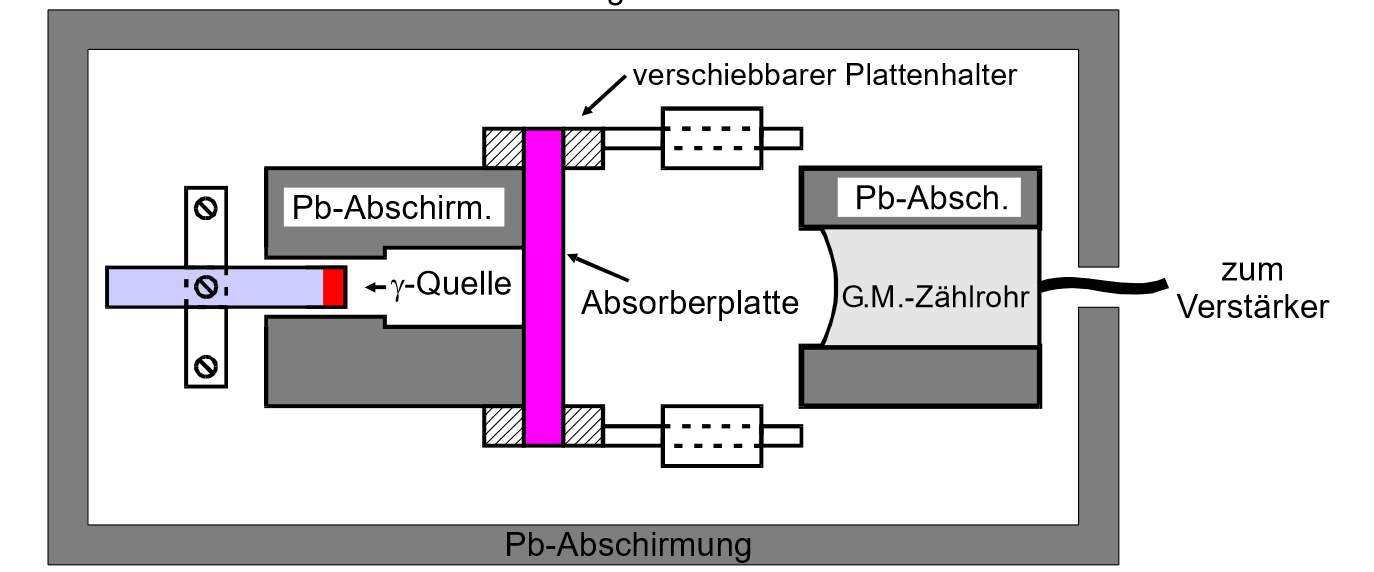
\includegraphics[width=\textwidth]{Bilder/Aufbau.png}
\caption{Abgebildet ist der schematische Aufbau zur Messung der Gamma-Strahlung}
\label{fig:Aufbau}
\end{figure}

Der Versuch wird wie in Abbildung \ref{fig:Aufbau} aufgebaut.
Zuerst wird die Anzahl der gemessenen Teilchen der Hintergrundstrahlung $N_{Hintergrund}$ über 900 Sekunden gemessen. 
Daraufhin wird eine Eisenplatte zwischen Quelle und Messgerät gestellt und abermals die Anzahl der Teilchen $N_E$ gemessen, hier mit einer Zeit von 60 Sekunden.
Dies wird für bis zu 13 verschiedene Dicken wiederholt, indem weitere Eisenplatten hinzugefügt werden.
Die Messung wird genau so für Aluminiumplatten durchgeführt. 

\subsection{Absorbtion von Beta-Strahlung}
Für $\beta^{-}$-Strahlung wird der Aufbau analog zu Abbildung \ref{fig:Aufbau} aufgebaut, nur der Gamma-Strahler wird durch einen Beta-Strahler ersetzt.
Dann wird eine Absorberplatte zwischen Strahler und Zählrohr gestellt, und die Anzahl der gemessenen Teilchen innerhalb von 60 Sekunden gemessen.
Die Platte wird mehrmals durch eine andere ausgetauscht, und die Messung wiederholt. 
Wenn wenig Impulse gemessen werden, wird die Messzeit erhöht.